\documentclass[miz,woman]{mgrwms}
\usepackage[utf8x]{inputenc}
\usepackage{amsfonts}
\usepackage{amsmath}
\usepackage[polish]{babel}
\usepackage[T1]{fontenc}
\usepackage{mathptmx}
\usepackage{array}
\usepackage{amsthm}



\title{ Twierdzenie Tur\`{a}na dla hipergrafów}
\author{ Agnieszka Walus}
\promotor{ prof zw. dr hab. Adam Paweł Wojda }
\nralbumu{ 124784 }
\slowakluczowe{ lista słów kluczowych w języku polskim }
\keywords{ lista słów kluczowych w języku angielskim }

\begin{document}
\newtheorem{defi}{Definicja}[section]
\newtheorem{tw}{Twierdzenie}[section]
\newtheorem{lem}[tw]{Lemat}
\theoremstyle{definition}
\newtheorem{przy}{Przykład}[section]


%---------------------------------RODZIAŁ I------------------------------------------------------
\chapter{Twierdzenie Tur\`{a}na dla grafów}
W rozdziale tym wprowadzimy podstawowe definicje związane z grafami, niezbędne do zrozumienia twierdzenia Tur\`{a}na.\\
\\
\section{Definicje}
Jeśli $V$ jest n-elementowym zbiorem to przez [$V$] oznaczać będziemy zbiór $\{$1,2, \dots ,n$\}$.
\begin{defi}
\textbf{Grafem prostym} lub \textbf{nieskierowanym} nazywamy uporządkowaną parę \\$G:=(V,E)$ gdzie:\\
\begin{itemize}
 \item $V$ jest niepustym zbiorem, którego elementy nazywamy \textbf{wierzchołkami}
 \item $E \subseteq$ [$V$]$^2$. Elementy z $E$ nazywamy \textbf{krawędziami}, a więc każda krawędź jest dwuelementowym
podzbiorem zbioru $V$. Krawędź $\{x,y\}$ często jest oznaczana przez $xy$.\\
Aby uniknąć niejasności zakłada się, że $E \cap V=\emptyset$.
\end{itemize}

\end{defi}

Jeśli będziemy mieć do czynienia z wieloma grafami, konieczne będzie zaznaczenie do którego grafu odnosi się oznaczenie
$V$ czy $E$.W tym celu mając na myśli graf $G$ jego zbiór wierzchołków oznaczymy przez $V(G)$, a zbiór krawędzi przez $E(G)$.\\
Liczbę wierzchołków w grafie oznaczamy przez |$V(G)$| i nazywamy \textbf{rzędem} grafu, a liczbę krawędzi oznaczamy przez 
||$E(G)$|| i nazywamy \textbf{rozmiarem} grafu.\\
\begin{defi}
 Mówimy, że wierzchołki $v$ i $w$ są \textbf{sąsiednie}, jeżeli w grafie istnieje krawędź łącząca $v$ i $w$.
\end{defi}
\begin{defi}
 Mówimy, że krawędź $e$ jest \textbf{incydentna} z wierzchołkiem $v$, jeśli $v \in e$.
\end{defi}
\begin {defi}
 \textbf{Stopniem} $d_G(v)$=$d(v)$ wierzchołka $v$ nazywamy liczbę krawędzi wychodzących z $v$. Inaczej: jest to liczba
 wierzchołków sąsiednich z $v$. Wierzchołek stopnia 0 nazywamy \textbf{izolowanym}.
\end {defi}
\begin{defi}
 Graf prosty, w którym każde dwa wierzchołki są sąsiednie nazywamy grafem \textbf{pełnym}. Graf pełny oparty na $n$ 
wierzchołkach oznaczamy przez $K_n$. Graf $K_3$ nazywamy \textbf{trójkątem}.
\end{defi}
\begin{defi}
Niech $G=(V,E)$, $H=(V',E')$ będą grafami. Jeśli $V'\subseteq V$ oraz $E'$ zawiera tylko takie krawędzie $xy\in E$, gdzie 
$x$,$y \in V'$, wtedy $H$ nazywamy podgrafem \textbf{indukowanym} (przez zbiór wierzchołków $V'$) i oznaczamy go $H:=G[V']$.
\end{defi}
\begin{defi}
 \textbf{Kliką} nazywamy podgraf, w którym każde dwa wierzchołki są połączone krawędzią. Inaczej:to podgraf, który jest 
grafem pełnym.
\end{defi}

\begin{defi}
 Graf którego zbiór wierzchołków można podzielić na $l$ parami rozłącznych podzbiorów (części) takich, że każde dwa wierzchołki
należące do tego samego podzbioru nie są połączone krawędzią nazywamy \textbf{$l$-dzielnym}.
\end{defi}


\section{Grafy Tur\`ana}
\begin{defi}
 \textbf{Grafem Tur\`ana} $T(n,l)$ nazywamy pełny $l$-dzielny graf oparty na $n\geq l$ wierzchołkach, przy czym liczność każdych
dwóch zbiorów podziału różni się co najwyżej o 1. 
\end{defi}
Dzieląc zbiór wierzchołków zgodnie z definicją grafu  Tur\`ana otrzymamy: $n \pmod l$ podzbiorów, które zawierają po $\lceil \frac{n}{l} \rceil$
elementów oraz $l-n\pmod l$ podzbiorów, które zawierają po $\lfloor \frac{n}{l} \rfloor$ elementów. Wierzchołki takiego grafu są stopnia $n-\lceil \frac{n}{l} \rceil$
albo $n- \lfloor \frac{n}{l} \rfloor$ a liczba jego krawędzi wynosi $\lfloor(1-\frac{1}{l}) \cdot \frac{n^2}{2} \rfloor$\\

\begin{przy}
Rozważmy graf Tur\`ana T(8,3), czyli $n$=8, $l$=3\\
$n\pmod l$  $\equiv $8$\pmod 3$=2 podzbiory, które zawierają po $\lceil \frac{8}{3} \rceil$=3 elementy\\
$l-n\pmod 3$ $\equiv $3-2 $\equiv $1 podzbiór, który zawiera $\lfloor \frac{8}{3} \rfloor$=2 elementy\\
Mamy więc 6 wierzchołków stopnia $n-\lceil \frac{n}{l} \rceil$=5 oraz 2 wierzchołki stopnia $n- \lfloor \frac{n}{l} \rfloor$=6.
Liczba krawędzi w $T(8,3)$ to $\lfloor(1-\frac{1}{l}) \cdot \frac{n^2}{2} \rfloor$=$\lfloor(1-\frac{1}{3}) \cdot \frac{8^2}{2}=21 \rfloor$
\begin{figure}[h]
\centering
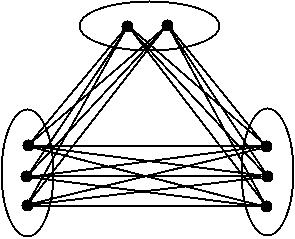
\includegraphics[width=5cm, height=5cm]{grafTurana.jpeg}
\end{figure}
\end{przy}

\begin{tw}
 Dla każdego $n$,$l$ każdy graf oparty na $n$ wierzchołkach, niezawierający  kliki $K_l$ i mający maksymalną
liczbę krawędzi jest grafem Tur\`ana T(n,l).
\end{tw}
Szczególnym przypadkiem powyższego twierdzenia (gdy $l$=2) jest twierdzenie Mantela:
\begin{tw}
 Maksymalna liczba krawędzi w grafie bez trójkątów jest równa co najwyżej $\lfloor \frac{n^2}{4} \rfloor$.
\end{tw}
\newpage

%-------------------------------ROZDZIAŁ II-----------------------------------------------------------------

\chapter{Twierdzenie Tur\`{a}na dla hipergrafów}
\section{Wprowadzenie do rozdziału}

Jeśli $V$ jest dowolnym zbiorem, to przez $|V|$ oznaczać będziemy liczność $V$ (liczbę elementów w $|V|$),
a przez $\mathcal{P}(V)$ zbiór wszystkich jego podzbiorów.\\
\begin{defi}
 \textbf{Hipergraf} jest uogólnieniem pojęcia grafu. To uporządkowana para \\
$H:=(V,E)$, gdzie:
\begin{itemize}
\item $V$ jest niepustym zbiorem, którego elementy nazywamy \textbf{wierzchołkami};
\item $E \subseteq \mathcal{P}(V)$. Elementy z $E$ nazywamy \textbf{hiperkrawędziami}, ale  dla ułatwienia nazywać je będziemy
po prostu krawędziami.
\end{itemize}
\end{defi}
Pojęcie hipergrafu utożsamiać będziemy ze zbiorem jego krawędzi. Mając na myśli zbiór wierzchołków hipergrafu, wyraźnie
to zaznaczymy. \\
\begin{defi}
 Dwa hipergrafy $H=(V,E)$ oraz $H'=(V',E')$ nazywamy \textbf{izomorficznymi}, jeśli istnieje bijekcja $f:V\rightarrow V'$
taka, że $\{x_1,x_2,\dots,x_n\} \in E \Longleftrightarrow \{f(x_1),f(x_2),\dots,f(x_n)\} \in E'$
\end{defi}

\begin{defi}
 Hipergraf nazywamy \textbf{r-jednolitym}, jeśli każda jego krawędź ma liczność r.\\
\end{defi}
Zauważmy, że hipergraf 2-jednolity to po prostu graf.
Dla uproszczenia r-jednolity hipergraf będziemy nazywać r-grafem.\\
\begin{defi}
 \textbf{Podhipergrafem }hipergrafu $G=(V,E)$ lub hipergrafem \textbf{indukowanym} przez zbiór wierzchołków $N$ nazywamy hipergraf $H=(N,E')$, gdzie
$N \subseteq V(H)$, $E'\subseteq E$ oraz w $E'$ znajdują się tylko takie krawędzie, które zawierają wyłącznie wierzchołki z $N$.\\
Dla ułatwnienia będziemy nazywać go po prostu podhipergrafem.\\
\end{defi}
\begin{defi}
 Niech $\mathcal{F}$ będzie dowolną rodziną $r$-grafów, a $G$ dowolnym $r$-grafem. Mówimy, że $G$ jest \textbf{{$\mathcal{F}$}-wolny},
jeśli nie zawiera żadnego elementu z $\mathcal{F}$ jako podhipergrafu.
\\
\end{defi}
Przez $ex(n,\mathcal{F})$ oznaczać będziemy maksymalną liczbę krawędzi w $n$ wierzchołkowym $r$-grafie $\mathcal{F}$-wolnym.\\
\begin{defi}
 Niech $l$,$r$ $\geq$2. Przez $K_l^{(r)}$ oznaczać będziemy rodzinę $r$-grafów z co najwyżej $l \choose 2$ krawędziami,
która zawiera zbiór wierzchołków $S$ zwany \textbf{rdzeniem} taki, że:
\begin{itemize}
 \item |$S$|=$l$
 \item każda para wierzchołków z $S$ jest zawarta w jakiejś krawędzi.
\end{itemize}
\end{defi}

Zauważmy, że gdy $r$=2 to nasza rodzina $K_l^{(r)}$ redukuje się do grafu pełnego $K_l$. Dla $r$>2 $K_l^{r}$ zawiera więcej niż jeden $r$-graf.
Dla ustalonego $r$ i $l$ rodzina $K_l^{(r)}$ jest skończona, bo każdy jej element ma co najwyżej $l \choose 2$ krawędzi.\\



\begin{defi}
  $r$-graf jest \textbf{$l$-dzielny}, jeśli zbiór jego wierzchołków można podzielić na $l$ podzbiorów (części) w taki sposób, aby
każda krawędź miała co najwyżej jeden wierzchołek w każdym podzbiorze.
W szczególności, gdy $l$<$r$, to $r$-graf nie ma krawędzi.\\
$l$-dzielny $r$-graf nazywamy \textbf{pełnym}, gdy wszystkie dozwolone krawędzie są obecne.
\end{defi}
\begin{defi}
Niech $n$,$l$,$r$ $\geq 1$. Pełny $l$-dzielny $r$-graf oparty na $n$ wierzchołkach nazywamy \textbf{hipergrafem Tur\`{a}na},
jeśli liczność każdych dwóch części podziału różni się co najwyżej o 1. Taki hipergraf oznaczamy przez $T_r(n,l)$.
\end{defi}

Poszczególne części mają liczności:
\begin{center}
 $n_i=\lfloor \frac{n+i-1}{l}\rfloor$ dla $i \in [l]$
\end{center}
Liczba krawędzi w $T_r(n,l)$ to:
\begin{center}
 $t_r(n,l)=\sum \limits_{S \in {[l] \choose r}} \prod \limits_{i \in S} n_i$
\end{center}
Spośród wszystkich $l$-dzielnych $r$-grafów opartych na $n$ wierzchołkach graf Tur\`{a}na $T_r(n,l)$ ma najwięcej krawędzi.\\
\begin{defi}
 Niech $G$ będzie dowolnym $r$-grafem, a $x,y\in V(G)$, $x \not =y$. Wtedy:\\
\begin{itemize}
 \item$L_G(x)=\{S-\{x\} : x \in S\in G\}$ nazywamy \textbf{połączeniem} wierzchołka $x$;\\
 \item$deg_G(x)=|L_G(x)|$ nazywamy \textbf{stopniem} wierzchołka x;\\
 \item$codeg_G(x,y)$ nazywamy \textbf{stopniem pary} x,y i jest to liczba krawędzi w $G$, które zawierają jednocześnie $x$ i $y$;\\
 \item$N_G(x)=\{z:codeg_G(x,z)>0\}$ nazywamy \textbf{sąsiedztwem} lub \textbf{zbiorem sąsiadów} wierzchołka $x$ w $G$.
\end{itemize}
\end{defi}
Jeśli wiemy którego hipergrafu dotyczą powyższe określenia, wtedy dla przejrzystości zapisu indeks $G$ można pominąć.
\section{Twierdzenie Tur\'ana}

\begin{lem} \label{lemat}
 Niech $n$ $\in \mathbb{N}$. Wtedy dla każdego $k \in [n]$ zachodzi:
\begin{equation}
t_r(n-k,l-1)+k \cdot t_{r-1}(n-k,l-1)\leq t_r(n,l) \label{nierownosc}
\end{equation}
Jeśli powyżej zachodzi równość, wtedy $k=\lfloor \frac{n}{l} \rfloor$ lub $k=\lceil \frac{n}{l} \rceil$.
\end{lem}
\begin{proof}
Niech $n$ $\in \mathbb{N}$. Dla każdego $k \in [n]$ lewą stronę nierówności można interpretować jako liczbę krawędzi w
następujacym hipergrafie: $T_r(n-k,l-1)$, do którego dokładamy $k$ wierzchołków, których połączenie jest hipergrafem
$T_{r-1}(n-k,l-1)$. Hipergrafy $T_r(n-k,l-1)$ i $T_{r-1}(n-k,l-1)$ oparte są na n-k wierzchołkach, które podzielone są
na $l-1$ części, z których liczność każdych dwóch różni się co najwyżej o 1. To wszystko oznacza, że  podział ich wierzchołków jest
taki sam. Dzięki temu na lewą stronę nierówności można patrzeć jak na liczbę krawędzi w pełnym $l$-dzielnym $r$-grafie, 
którego każde dwie części spośród $l-1$ różnią się licznością o co najwyżej 1, a ostatnia $l$-ta część ma liczność $k$.
Jak już wcześniej zostało wspomniane, $T_r(n,l)$ maksymalizuje rodzinę pełnych $l$-dzielnych $r$-grafów, więc lewa strona
nierówności jest mniejsza od liczby krawędzi takiego hipergrafu oznaczanej przez $t_r(n,l)$. Jeśli w (2.1) będzie zachodzić
równość, będzie to oznaczało, że $n$ wierzchołków zostało podzielonych na $l$ możliwie równych części, więc każde dwie części
będą się różniły o co najwyżej jeden wierzchołek, a to oznacza, że ostatnia ($l$-ta) część musi mieć liczność 
$\lfloor \frac{n}{l} \rfloor$ lub $\lceil \frac{n}{l} \rceil$.
\end{proof}
Warto zastanowić się, jak będzie wyglądał powyższy lemat gdy $l=r$. Ponieważ r>l-1, więc hipergraf $T_r(n-k,l-1)$ nie
będzie posiadał żadnej krawędzi, dlatego naszą nierówność można zredukować do:
\begin{equation}
k \cdot t_{r-1}(n-k,l-1)\leq t_r(n,l)
\end{equation}
Jeżeli powyżej będzie zachodzić równość, wtedy podobnie jak w dowodzie lematu, ostatnia $l$-ta część podziału zbioru wierzchołków
musi mieć liczność $\lfloor \frac{n}{l} \rfloor$ lub $\lceil \frac{n}{l} \rceil$.

\end{document}
